% use the "wcp" class option for workshop and conference
% proceedings
%\documentclass[gray]{jmlr} % test grayscale version
%\documentclass[tablecaption=bottom]{jmlr}% journal article
\documentclass[pmlr,twocolumn,10pt]{jmlr} % W&CP article

% REQUIRED: select your submission track. Use one of:
  %   proceedings, findings, demo, perspective
  % Leaving the argument empty (\mlhtrack{}) compiles but shows a red
  % "please specify the submission track" warning in the page header.
  % Removing this line entirely raises a "No ML4H track specified" class error.
  % NOTE: keep \mlhtrack{...} BEFORE the \iffinal / \ifmlhneedspmlr blocks below —
  % those conditionals depend on the flags this command sets.
\mlhtrack{findings}

\newif\iffinal
\finalfalse  % toggle this flag for initial submission
% \finaltrue  % toggle this flag for camera-ready version after acceptance

\iffinal
    % For Proceedings and Perspective tracks (published in PMLR), replace XXX below
    % with the specific PMLR volume number sent to you before the camera-ready submission.
    \ifmlhneedspmlr
      \jmlrvolume{XXX}
      \jmlryear{2026}
    \fi
    \ifmlhfindings \jmlrproceedings{}{ML4H 2026 - Findings Track}\fi
    \ifmlhdemo     \jmlrproceedings{}{ML4H 2026 - Demo Track}\fi
    \jmlrworkshop{Machine Learning for Health (ML4H) 2026}
\else
    % Submitted for review
    \jmlrproceedings{}{Submitted to ML4H 2026: \mlhtrackname}
    \jmlrworkshop{Machine Learning for Health (ML4H) 2026}
\fi

% \usepackage{geometry}
% \geometry{margins=0.1in,textwidth=7in}

% The following packages will be automatically loaded:
% amsmath, amssymb, natbib, graphicx, url, algorithm2e
\urlstyle{same}

%\usepackage{rotating}% for sideways figures and tables
%\usepackage{longtable}% for long tables

% The booktabs package is used by this sample document
% (it provides \toprule, \midrule and \bottomrule).
% Remove the next line if you don't require it.

\usepackage{booktabs}
% The siunitx package is used by this sample document
% to align numbers in a column by their decimal point.
% Remove the next line if you don't require it.
\usepackage{siunitx}

% The lineno package is required for denoting line
% numbers for paper review.
\usepackage[switch]{lineno}

% The following command is just for this sample document:
\newcommand{\cs}[1]{\texttt{\char`\\#1}}% remove this in your real article

% The following is to recognise equal contribution for authorship
\newcommand{\equal}[1]{{\hypersetup{linkcolor=black}\thanks{#1}}}

% Define an unnumbered theorem just for this sample document for
% illustrative purposes:
\theorembodyfont{\upshape}
\theoremheaderfont{\scshape}
\theorempostheader{:}
\theoremsep{\newline}
\newtheorem*{note}{Note}

% The optional argument of \title is used in the header
\title[Plan-Then-Compile]{Plan-Then-Compile: Resolving Clinical Terminology
in the Database Enables FHIR-to-SQL Generalization to Unseen Concepts}

% Anything in the title that should appear in the main title but 
% not in the article's header or the volume's table of
% contents should be placed inside \titletag{}

%\title{Title of the Article\titletag{\thanks{Some footnote}}}


% Use \Name{Author Name} to specify the name.
% If the surname contains spaces, enclose the surname
% in braces, e.g. \Name{John {Smith Jones}} similarly
% if the name has a "von" part, e.g \Name{Jane {de Winter}}.
% If the first letter in the forenames is a diacritic
% enclose the diacritic in braces, e.g. \Name{{\'E}louise Smith}

% \thanks must come after \Name{...} not inside the argument for
% example \Name{John Smith}\nametag{\thanks{A note}} NOT \Name{John
% Smith\thanks{A note}}

% Anything in the name that should appear in the title but not in the 
% article's header or footer or in the volume's
% table of contents should be placed inside \nametag{}

% Anonymized author list during review
\author{Anonymous Author(s)}

% Two authors with the same address
% \author{%
%  \Name{Author Name1\nametag{\thanks{A note}}} \Email{abc@sample.com}\and
%  \Name{Author Name2} \Email{xyz@sample.com}\\
%  \addr Address
% }

% Three or more authors with the same address:
% \author{%
%  \Name{Author Name1} \Email{an1@sample.com}\\
%  \Name{Author Name2} \Email{an2@sample.com}\\
%  \Name{Author Name3} \Email{an3@sample.com}\\
%  \Name{Author Name4} \Email{an4@sample.com}\\
%  \Name{Author Name5} \Email{an5@sample.com}\\
%  \Name{Author Name6} \Email{an6@sample.com}\\
%  \Name{Author Name7} \Email{an7@sample.com}\\
%  \Name{Author Name8} \Email{an8@sample.com}\\
%  \Name{Author Name9} \Email{an9@sample.com}\\
%  \Name{Author Name10} \Email{an10@sample.com}\\
%  \Name{Author Name11} \Email{an11@sample.com}\\
%  \Name{Author Name12} \Email{an12@sample.com}\\
%  \Name{Author Name13} \Email{an13@sample.com}\\
%  \Name{Author Name14} \Email{an14@sample.com}\\
%  \addr Address
% }

% % Authors with different addresses and equal first authors:
% \author{%
% \Name{First Author 1}\equal{These authors contributed equally} \Email{abc@sample.com}\\
% \addr University X, Country 1
% \AND
% % footnotemark[1] is to refer to the \equal footnote
% \Name{First Author 2}\footnotemark[1] \Email{def@sample.com}\\
% \addr University Y, Country 2
% \AND
% \Name{Last Author} \Email{ghi@sample.com}\\
% \addr University Z, Country 3
% }

%%%%%%%%%%%%%%%%%%%%%%%%%%%%%%%%%%%%%%%%%%%%%%%%%%%%%%%%%%%%%%%%%%%%%%%%
%%%%%%%%%%%%% Remove the \linenumbers in the final version %%%%%%%%%%%%%
%%%%%%%%%%%%%%%%%%%%%%%%%%%%%%%%%%%%%%%%%%%%%%%%%%%%%%%%%%%%%%%%%%%%%%%%
\linenumbers % Activate line numbering

\begin{document}

\maketitle

\ifmlhdemo\else
\begin{abstract}
Text-to-SQL over clinical data conflates two skills: composing a query, and
mapping a clinical concept to the code the database stores it under. When gold
SQL embeds literal codes, the second is memorization, and no metric computed on
that data can separate them. We rebuild a FHIR-derived benchmark so terminology
is resolved \emph{through the database} --- every gold query looks the concept up
in a \texttt{valuesets} table at runtime and never embeds a literal SNOMED CT,
ICD-10 or RxNorm code --- and pair each target with a structured JSON query plan
compiled into SQL in one completion. On an earlier version of this pipeline that
did embed literal codes, a fine-tuned model reached 98.4\% execution match on
familiar concepts but 20.7\% on concepts absent from training. Under the lookup
design, DoRA fine-tuning of a 14B open-weight coder model reaches 100\% on
familiar concepts and 89.1\% on unseen ones (81.4\% by the stricter text metric),
from frozen baselines of 34.8\% and 60.8\%. An ablation isolates why this works:
merely making the lookup table \emph{visible} in the schema drives the
\emph{untrained} model's code-hardcoding from 3.4\% to 0.0\%, with no training
signal at all --- models bypass a resolution mechanism they cannot see. We
additionally report that a DAPO/GRPO stage adds nothing on top of supervised
fine-tuning, which already saturates the reward's correctness gate.
\end{abstract}
\begin{keywords}
text-to-SQL, clinical natural language processing, electronic health records,
FHIR, large language models, parameter-efficient fine-tuning, clinical
terminology, synthetic health data
\end{keywords}
\fi

\ifmlhneedsstatements
\paragraph*{Data and Code Availability}
This study uses only synthetic patient records generated by Synthea
\citep{walonoski2018synthea}; no real patient data is involved. The corpus
comprises two disjoint synthetic populations (18,999 training and 6,383 held-out
patients) flattened into a relational schema. All code, generated datasets,
trained adapter weights, and the complete per-seed training logs, evaluation
summaries, failure logs and ablation results behind every number reported here
are publicly released under open licenses. An anonymized copy of the generation
and analysis code, the schema, the training notebooks, and all per-seed logs and
evaluation results accompanies this submission as supplementary material. Public
links are withheld here to preserve anonymity and will be provided on acceptance.

\paragraph*{Institutional Review Board (IRB)}
This research does not require IRB approval. It uses only synthetic patient
records generated by Synthea and involves no human subjects, no real patient
data, and no identifiable information.
\fi

\section{Introduction}
\label{sec:intro}

``How many patients with essential hypertension were prescribed a statin last
year?'' looks like one translation step. It decomposes into at least four:
isolating the clinical entities, identifying the query archetype they imply,
composing SQL over a normalized schema, and resolving each concept to the code
the data actually uses. The first three are reasoning that should transfer. The
fourth, done from parametric memory, is recall --- it degrades for rare concepts,
varies across coding systems (SNOMED CT, ICD-10, RxNorm, LOINC, CDT and CVX all
appear in our corpus), and cannot be audited.

Conventional supervision collapses all four into an opaque mapping to a query
string, which is a measurement problem as much as a capability one: when a model
is wrong there is no way to tell which skill failed, and when it is right there
is no way to tell whether it reasoned or recognized.

This is not hypothetical. An earlier iteration of our own pipeline embedded
literal codes in gold SQL. A fine-tuned model then reached 98.4\% execution match
on familiar clinical concepts and \textbf{20.7\%} on concepts absent from
training --- not a reasoning failure, but a model unable to know codes it had
never been shown. Rebuilding the corpus around database-resolved terminology is
the response, and the results below are the comparison.

Clinical text-to-SQL has an established line of work
\citep{wang2020mimicsql,lee2022ehrsql,lee2024trustsql}, as do intermediate
representations between question and query
\citep{guo2019irnet,wang2020ratsql,pourreza2023dinsql} and cross-domain
benchmarks \citep{yu2018spider,li2023bird}. Our contribution is not a new
learning algorithm but a corpus and evaluation design that makes one specific
capability --- generalization to clinical concepts absent from training ---
separable and measurable.

\paragraph{Contributions.}
(i) A FHIR-native corpus in which terminology resolution is a queryable
operation rather than recall, with an evaluation design that isolates
generalization to unseen clinical concepts from generalization to unseen
patients. (ii) A soundness-by-construction detector for lookup bypass, and the
finding that schema \emph{visibility} alone eliminates hardcoding in an
untrained model. (iii) An explicit accounting of how much of each evaluation arm
is genuinely novel, and a quantified bound on how discriminative execution match
actually is. (iv) A scoped null result with mechanism: once supervised
fine-tuning saturates the reward's correctness gate, a DAPO/GRPO stage
\citep{yu2025dapo,shao2024deepseekmath} has nothing left to optimize.

\section{Method}

\subsection{Terminology resolved in the database}

Every coded table carries a \texttt{code}/\texttt{system}/\texttt{display}
triple, and a \texttt{valuesets} table indexes every
\texttt{(table\_name, code, code\_system, display)} combination in the corpus.
Gold SQL never contains a literal clinical code; it resolves the concept at query
time, as in:

\begin{small}
\begin{verbatim}
WITH resolved AS (
  SELECT code, code_system FROM valuesets
  WHERE table_name = 'procedure'
    AND display ILIKE '%Depression screening%'
)
SELECT DISTINCT patient_id
FROM procedure, resolved
WHERE procedure.code = resolved.code
  AND procedure.system = resolved.code_system
  AND status = 'completed'
\end{verbatim}
\end{small}

This needs no retrieval infrastructure, no tool calls and no prompt-format
change --- it is ordinary SQL over columns that already exist. The model need
only produce a plausible search phrase; the database resolves it
deterministically. Concepts whose display text matches more than one row are
excluded from gold generation rather than resolved by an arbitrary tiebreak.

\subsection{Plan, then compile}

Each target is a structured JSON query plan followed by the compiled SQL in one
continuous completion. The plan's \texttt{entities} array names the concepts,
their roles (primary vs.\ companion), clinical domain, and whether each needs a
lookup; \texttt{constraints} and \texttt{aggregation} encode the archetype, drawn
from a closed vocabulary where every value maps to a clause shape some template
already needs. Because the plan precedes the SQL autoregressively, the model
commits to its reading of the question before composing the query, and that
commitment is recoverable from the output.

\subsection{Detecting lookup bypass}

A model could still embed a literal code and produce a correct query, which an
execution-only metric cannot see. We flag any comparison of
\texttt{code}/\texttt{system} (and their FHIR-prefixed variants) against a quoted
literal. This is sound by construction: legitimate lookup CTEs filter only on
\texttt{table\_name} and \texttt{display}, and join against \emph{identifiers},
never literals, so a match can only mean the lookup was bypassed. Validated
against all 9,680 gold-SQL-bearing training rows with zero false positives.

\section{Setup}

Two disjoint synthetic populations were generated with Synthea
\citep{walonoski2018synthea} (train 18,999 patients; held-out 6,383; zero
\texttt{patient\_id} overlap, verified by set intersection). Questions come from
an archetype $\times$ concept factory: 82 archetypes (64 answerable, 18
unanswerable) across four difficulty tiers plus operational, regulatory and
quality-KPI categories, instantiated against concepts spanning the coverage
range. Every answerable gold query was executed and kept only if it ran without
error and returned at least one row, then checked for repeated-execution
stability. Assembled: 10,696 training rows (9,680 execution-verified $+$ 1,016
unanswerable), 2,420 distinct gold queries.

We fine-tune \texttt{Qwen2.5-Coder-14B-Instruct} \citep{hui2024qwen25coder} with
DoRA \citep{liu2024dora} (rank 16, $\alpha$ 32, all linear layers) under NF4
quantization \citep{dettmers2023qlora}, two epochs, three seeds, on a single
consumer-cloud GPU ($\approx$12\,h/seed). A DAPO stage \citep{yu2025dapo} then
continues each seed's best checkpoint. All queries execute against DuckDB
\citep{raasveldt2019duckdb}.

\paragraph{Two evaluation arms.} \emph{Familiar} --- concepts also used in
training, against the disjoint population, isolating \emph{population}
generalization. \emph{Unseen} --- 84 concepts appearing nowhere in training
(verified disjoint; zero shared question/query pairs), isolating \emph{concept}
generalization.

\begin{figure}[t]
\centering
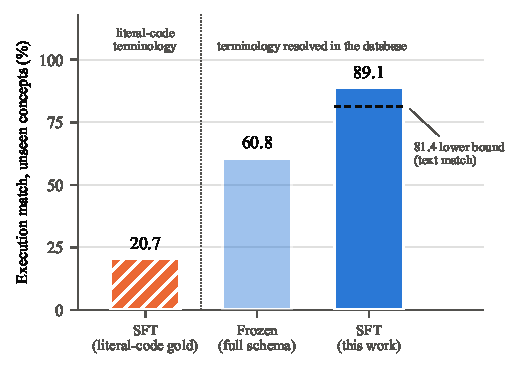
\includegraphics[width=\linewidth]{fig1_unseen}
\caption{Execution match on clinical concepts absent from training. Left: an
earlier iteration of this same pipeline, in which gold SQL embedded literal
clinical codes. Right: the database-resolved design, frozen and fine-tuned, both
given the complete schema. The dashed line marks the 81.4\% lower bound implied
by the stricter text-match metric (Section~\ref{sec:arms}).}
\label{fig:unseen}
\end{figure}

\section{Results}

\begin{table}[t]
\centering
\small
\caption{Held-out benchmark, mean over three seeds. Frozen figures use a
\emph{complete} schema description (Section~\ref{sec:abl}); under the
training-time prompt they are 10.2\% and 31.3\%.}
\label{tab:main}
\begin{tabular}{lrrr}
\toprule
 & Frozen & SFT & SFT+RL \\
\midrule
Exec.\ match, familiar & 34.8 & \textbf{100.0} & 100.0 \\
Exec.\ match, unseen   & 60.8 & \textbf{89.1}  & 89.2 \\
Text match, unseen     & 0.0  & 81.4  & 81.5 \\
Hardcoding rate        & 0.0  & 0.0   & 0.0 \\
\bottomrule
\end{tabular}
\end{table}

Table~\ref{tab:main} gives the headline, and Figure~\ref{fig:unseen} isolates the
effect of the terminology design on the arm that matters. A frozen model given
the full schema still never reproduces a gold query (0.0\% text match on both
arms), refuses unanswerable questions unreliably in both directions, and writes
correct queries 4.5--12$\times$ slower than gold. After fine-tuning, familiar-arm
execution correctness is perfect on all three seeds; the unseen arm reaches
89.1\% (85.0--92.1\% across seeds).

\subsection{Ablation: schema visibility alone removes hardcoding}
\label{sec:abl}

During our published runs the schema shipped to the model omitted the
\texttt{valuesets} DDL: fine-tuned models had learned the table's shape from
training targets, but the frozen baseline had only the table name. We re-ran the
frozen model twice on identical rows, with and without that DDL.

Showing it the table quadruples familiar-arm execution match
(8.7\%\,$\rightarrow$\,34.8\%) and roughly doubles unseen
(31.2\%\,$\rightarrow$\,60.8\%). A fine-tuned control moves $+0.8$\,pp,
confirming those models had already internalized the schema. Most striking:
terminology-hardcoding falls to \textbf{0.0\%} on both arms (from 1.8\% and
4.2\%). \emph{An untrained model stops embedding literal codes purely because the
lookup route became discoverable.} Models bypass a resolution mechanism they
cannot see; the fix is as much schema design as training. The event counts are
small (6 hardcoded completions across the without-DDL legs), so we report
direction rather than effect size.

\subsection{A scoped null: RL adds nothing once SFT saturates the objective}

All three seeds hit their best dev execution match at the \emph{first}
evaluation checkpoint (step 10) and never improved, early-stopping at step 40 of
a 200-step budget. Mean reward sat at or above 1.0 --- the correct-answer floor
--- on 37--38 of 40 steps, meaning sampled completions were already
overwhelmingly correct before any update. With correctness saturated, the reward
variance Dynamic Sampling retained (it still kept $\approx$87\% of groups) must
have come largely from the small efficiency bonus, which is derived from
wall-clock timing. We did not log per-group reward components, so this is an
inference from reward statistics rather than a measurement.

\section{What each arm can and cannot show}
\label{sec:arms}

We report this explicitly because the headline invites over-reading.
\textbf{96.5\%} of the familiar arm's answerable rows are byte-identical
(question, gold SQL) pairs from training; only the patient population differs,
and gold SQL holds no patient-specific literals. A purely memorizing model would
also score 100\% there. That arm shows learned queries \emph{stay correct} on new
data --- necessary, not sufficient. The unseen arm shares zero question/query
pairs and zero concepts with training, and is where transfer is established.

Its 89.1\% is an \textbf{upper bound}. Unseen concepts are rare (1--3 patients
each) and gold answers are small integers, so \textbf{53.9\%} of within-archetype
concept pairs return identical results --- confusing one concept for another can
go undetected. Text-match metrics cannot be satisfied that way and give 81.4\% as
a lower bound. True performance lies in 81--89\%.

Finally, the 1,016 unanswerable questions are identical across training and both
arms, so perfect abstention measures \emph{retention} of trained refusal, not
held-out refusal generalization.

\section{Discussion}

\paragraph{Why not simply call a frontier API?} We deliberately do not benchmark
against proprietary hosted models. For the deployment this targets --- querying
PHI-bearing clinical databases --- transmitting records to a third-party API is
frequently precluded by data-governance and residency rules regardless of
accuracy, so a hosted baseline would not be an available alternative even if it
matched. The relevant comparison is against what can run inside the
institution's own boundary. A locally hosted adapter also has bounded, one-off
cost rather than per-query billing.

\paragraph{Limitations.} Synthetic data only; all questions derive from one
templated generation distribution, so robustness to free-form clinician phrasing
is untested; terminology resolution is substring matching over a dictionary with
one display string per code, so synonymy, hierarchy and genuine ambiguity are out
of scope (ambiguous concepts are excluded from gold) --- real deployment needs
value-set expansion; a single base model, scale and schema; and the unseen arm's
archetypes are all trained archetypes, so what transfers is concept
identification and lookup composition, not novel query composition.

\paragraph{Outlook.} Nothing here is specific to FHIR. Any domain with a
normalized schema, a controlled vocabulary and a supply of verifiable queries
presents the same structure. The most useful extension is not a larger model but
a harder benchmark with genuine headroom above the supervised ceiling --- which
is where an RL stage might finally earn its cost.

\bibliography{refs}

\end{document}
